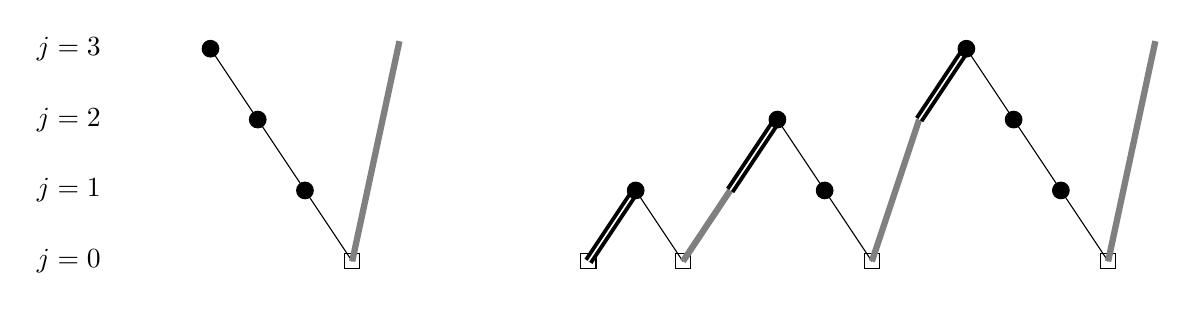
\begin{tikzpicture}[scale=1.2]
  \pgfmathsetmacro\hstep{0.5}
  \pgfmathsetmacro\vstep{0.75}
  \pgfmathsetmacro\ceps{0.08}   % size of square for coarse grid

% grid labels at left
  \node at (-6,3*\vstep) {$j=3$};
  \node at (-6,2*\vstep) {$j=2$};
  \node at (-6,\vstep) {$j=1$};
  \node at (-6,0.0) {$j=0$};

% 4-level slash-cycle
  \draw[black,thin] (-9*\hstep,3*\vstep) -- (-8*\hstep,2*\vstep) -- (-7*\hstep,\vstep) --  (-6*\hstep,0.0);
  \filldraw (-9*\hstep,3*\vstep) circle (2.5pt);
  \filldraw (-8*\hstep,2*\vstep) circle (2.5pt);
  \filldraw (-7*\hstep,\vstep) circle (2.5pt);
  \draw     (-6*\hstep-\ceps,-\ceps) rectangle (-6*\hstep+\ceps,+\ceps);
  \draw[gray,line width=0.8mm] (-6*\hstep,0.0) -- (-5*\hstep,3*\vstep+\ceps);

% coarse solve only
  \draw     (-\hstep-\ceps,-\ceps) rectangle (-\hstep+\ceps,+\ceps);
  \draw[black,double,line width=0.5mm] (-\hstep,0.0) -- (0.0,\vstep);
% 2-level slash-cycle
  \draw[black,thin] (0.0,\vstep) -- (\hstep,0.0);
  \filldraw (0.0,\vstep) circle (2.5pt);
  \draw     (\hstep-\ceps,-\ceps) rectangle (\hstep+\ceps,+\ceps);
  \draw[gray,line width=0.8mm] (\hstep,0.0) -- (2*\hstep,\vstep);
  \draw[black,double,line width=0.5mm] (2*\hstep,\vstep) -- (3*\hstep,2*\vstep);
% 3-level slash-cycle
  \draw[black,thin] (3*\hstep,2*\vstep) -- (4*\hstep,\vstep) --  (5*\hstep,0.0);
  \filldraw (3*\hstep,2*\vstep) circle (2.5pt);
  \filldraw (4*\hstep,\vstep) circle (2.5pt);
  \draw     (5*\hstep-\ceps,-\ceps) rectangle (5*\hstep+\ceps,+\ceps);
  \draw[gray,line width=0.8mm] (5*\hstep,0.0) -- (6*\hstep,2*\vstep);
  \draw[black,double,line width=0.5mm] (6*\hstep,2*\vstep) -- (7*\hstep,3*\vstep);
% 4-level slash-cycle
  \draw[black,thin] (7*\hstep,3*\vstep) -- (8*\hstep,2*\vstep) -- (9*\hstep,\vstep) --  (10*\hstep,0.0);
  \filldraw (7*\hstep,3*\vstep) circle (2.5pt);
  \filldraw (8*\hstep,2*\vstep) circle (2.5pt);
  \filldraw (9*\hstep,\vstep) circle (2.5pt);
  \draw     (10*\hstep-\ceps,-\ceps) rectangle (10*\hstep+\ceps,+\ceps);
  \draw[gray,line width=0.8mm] (10*\hstep,0.0) -- (11*\hstep,3*\vstep+\ceps);

\end{tikzpicture}
